\documentclass{article}
\usepackage[utf8]{inputenc}
\usepackage{graphicx}
\usepackage{amsmath}
\usepackage[margin=1.0in]{geometry}
\usepackage{float}
\usepackage{hyperref}
\usepackage{subcaption}
\usepackage{listings}
\usepackage{color}
\usepackage{enumerate}
\usepackage{enumitem}
\usepackage{caption}
\usepackage{hhline}
\usepackage{tabularx}



\title{Predicting COMPASS/AMBER Acceptance with Neural Networks}
\author{Pedro M. P. Curvo}
\date{\today}

\begin{document}
\maketitle

\section{Introduction}

\subsection{COMPASS/AMBER}

The COMPASS experiment, short for "Common Muon and Proton Apparatus for Structure 
and Spectroscopy," is a cutting-edge particle physics experiment conducted at CERN, 
the European Organization for Nuclear Research, in Geneva, Switzerland. COMPASS is a 
collaborative endeavor involving scientists and researchers from institutions around the world.
This experiment is dedicated to unraveling the mysteries of the subatomic world by probing the 
structure and properties of hadrons, which are particles composed of fundamental constituents 
called quarks and held together by the strong nuclear force. COMPASS achieves this by utilizing 
a high-energy polarized muon beam, making it unique in its precision measurements of hadron 
physics and spin properties.
With its sophisticated array of detectors, including spectrometers and tracking chambers, 
COMPASS captures and analyzes particles produced during high-energy collisions, providing 
valuable insights into the internal structure of nucleons like protons and neutrons. 
Additionally, COMPASS explores the production of exotic hadrons, expanding our understanding 
of the strong force interactions and the fundamental constituents of matter.
The data generated by the COMPASS experiment contributes significantly to advancing our 
knowledge of the building blocks of the universe and the forces that govern them, 
furthering our understanding of the intricacies of particle physics.


\section{Data Origin and Preprocessing}

\subsubsection*{Data Origin: Generation and Reconstruction}
The data used for the analysis presented in this paper was generated using a LEPTO generator,
a dedicated generator for deep inelastic scattering (DIS) processes. Beyond that, the full simulation
of the COMPASS spectrometer was done using the GEANT4 programme. The data was then reconstructed
using the COMPASS reconstruction software. With this process, two files were generated for each type of events (Hadrons and Inclusive), one with the
Monte Carlo (MC) data, and another with the reconstructed data. 
The goal with this data is to check if it is possible to predict the acceptance of the COMPASS/AMBER
using a Neural Network, since the GEANT4 simulation is very time consuming, aproximately 30 seconds per event.
That might not seem like a lot, but when you have millions of events, it becomes a problem.
Therefore, one could use a Neural Network to habe a better idea of how changed parameters affect the data/MC
agreement, and then only run the GEANT4 simulation for the events that are more likely to be accepted.


\subsubsection*{Data Variables}
The data used for the analysis of the Inclusive events has 11 variables:

\begin{table}[H]
    \centering
    \begin{tabular}{c|l}
    \textbf{Variable} & \textbf{Description} \\ \hline
    $X_b$ & $Bjorken_x$ \\
    $Y$ & Virtual Photon Energy Fraction of the initial momentum\\
    $Q^2$ & Four-momentum transfer \\
    $Trig$ & Trigger \\
    $PV_z$ & X-Position of interaction vertex in the target\\
    $PV_x$ & Y-Position of interaction vertex in the target\\
    $PV_y$ & Z-Position of interaction vertex in the target\\
    $Mom_{mu}$ & Incoming beam momentum\\
    $Mom_{mup}$ & Outgoing muon momentum\\
    $d_xd_zmup$ & Angle of Muon \\
    $d_yd_zmup$ & Angle of Muon \\
    \end{tabular}
\end{table}

While the data used for the analysis of the Hadrons events has 16 variables:

\begin{table}[H]
    \centering
    \begin{tabular}{c|l}
    \textbf{Variable} & \textbf{Description} \\ \hline
    $X_b$ & $Bjorken_x$ \\
    $Y$ & Virtual Photon Energy Fraction of the initial momentum\\
    $Z$ & Fraction of hadron energy to the virtual photon energy \\
    $Q^2$ & Four-momentum transfer \\
    $Trig$ & Trigger \\
    $PV_z$ & X-Position of interaction vertex in the target\\
    $PV_x$ & Y-Position of interaction vertex in the target\\
    $PV_y$ & Z-Position of interaction vertex in the target\\
    $Mom_{mu}$ & Incoming beam momentum\\
    $Mom_{mup}$ & Outgoing muon momentum\\
    $d_xd_zmup$ & Angle of Muon \\
    $d_yd_zmup$ & Angle of Muon \\
    $q$ & Hadron Charge \\
    $mom$ & Momentum of Hadron \\
    $d_xd_z$ & Angle of Hadron \\
    $d_yd_z$ & Angle of Hadron \\
    \end{tabular}
\end{table}



As mentioned before, for each type of events, we have a file with the Monte Carlo data and another with the reconstructed data.
Since the goal is to find a way to predict the acceptance of the COMPASS/AMBER, we created a new variable, called "Accepted",
which is 1 if the event was accepted and 0 if it was rejected. Therefore, for the data with the Monte Carlo information, we added
a column with the value 1 for all the events, and for the data with the reconstructed information, we added a column with the value 0.
It's important to refer that the number of events for each of the files is different, since the Monte Carlo data has more events than the reconstructed data.
Hence, we had to balance the data for the training and testing of the Neural Network, which will be explained in the section.


\subsubsection*{Correlation between Variables}
In order to check if there is any correlation between the variables, we plotted the correlation matrix for the Inclusive and Hadrons events.
This is important because if there is a high correlation between two variables, it means that they are redundant, and therefore, one of them can be removed, 
which simplifies the training of the Neural Network, reduces the number of parameters (reducing the training time) and avoids overfitting.
The results are shown in the figures below:

\begin{figure}[H]
    \centering
    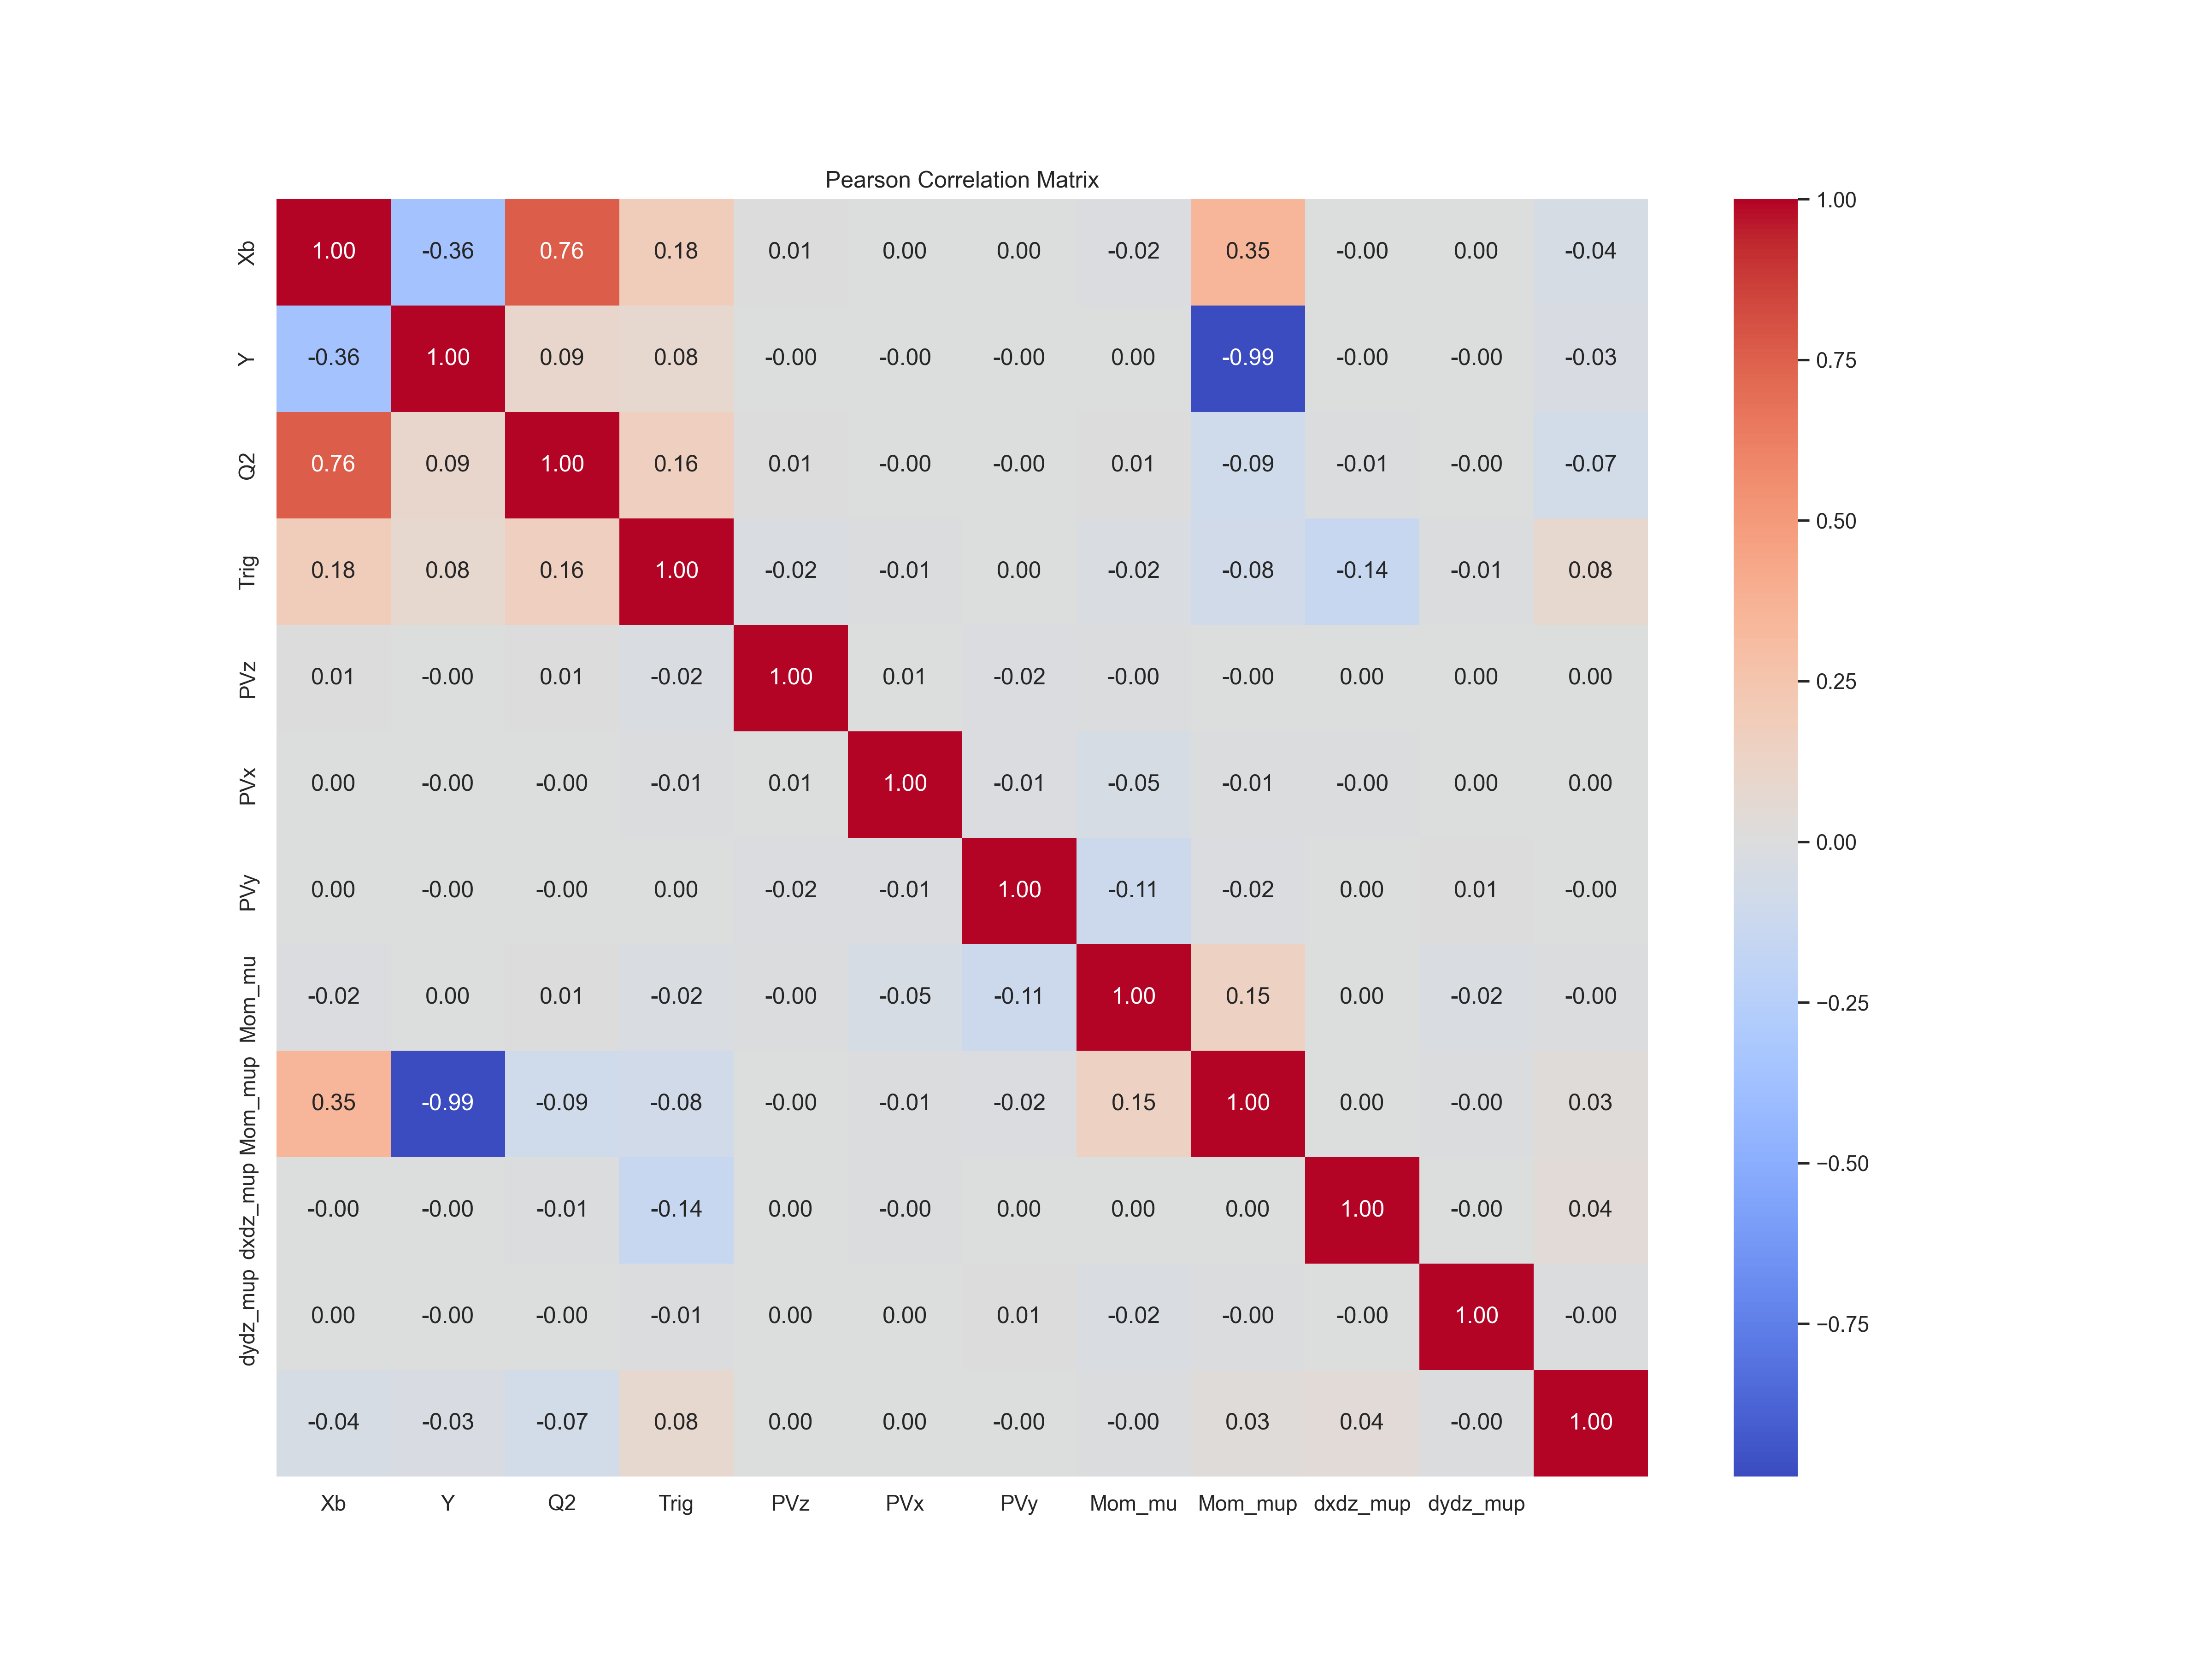
\includegraphics[width=0.9\textwidth]{graphs/inclusive_correlation_matrix.png}
    \caption{Correlation Matrix for the Inclusive Events}
    \label{fig:inclusive_correlation_matrix}
\end{figure}

\begin{figure}[H]
    \centering
    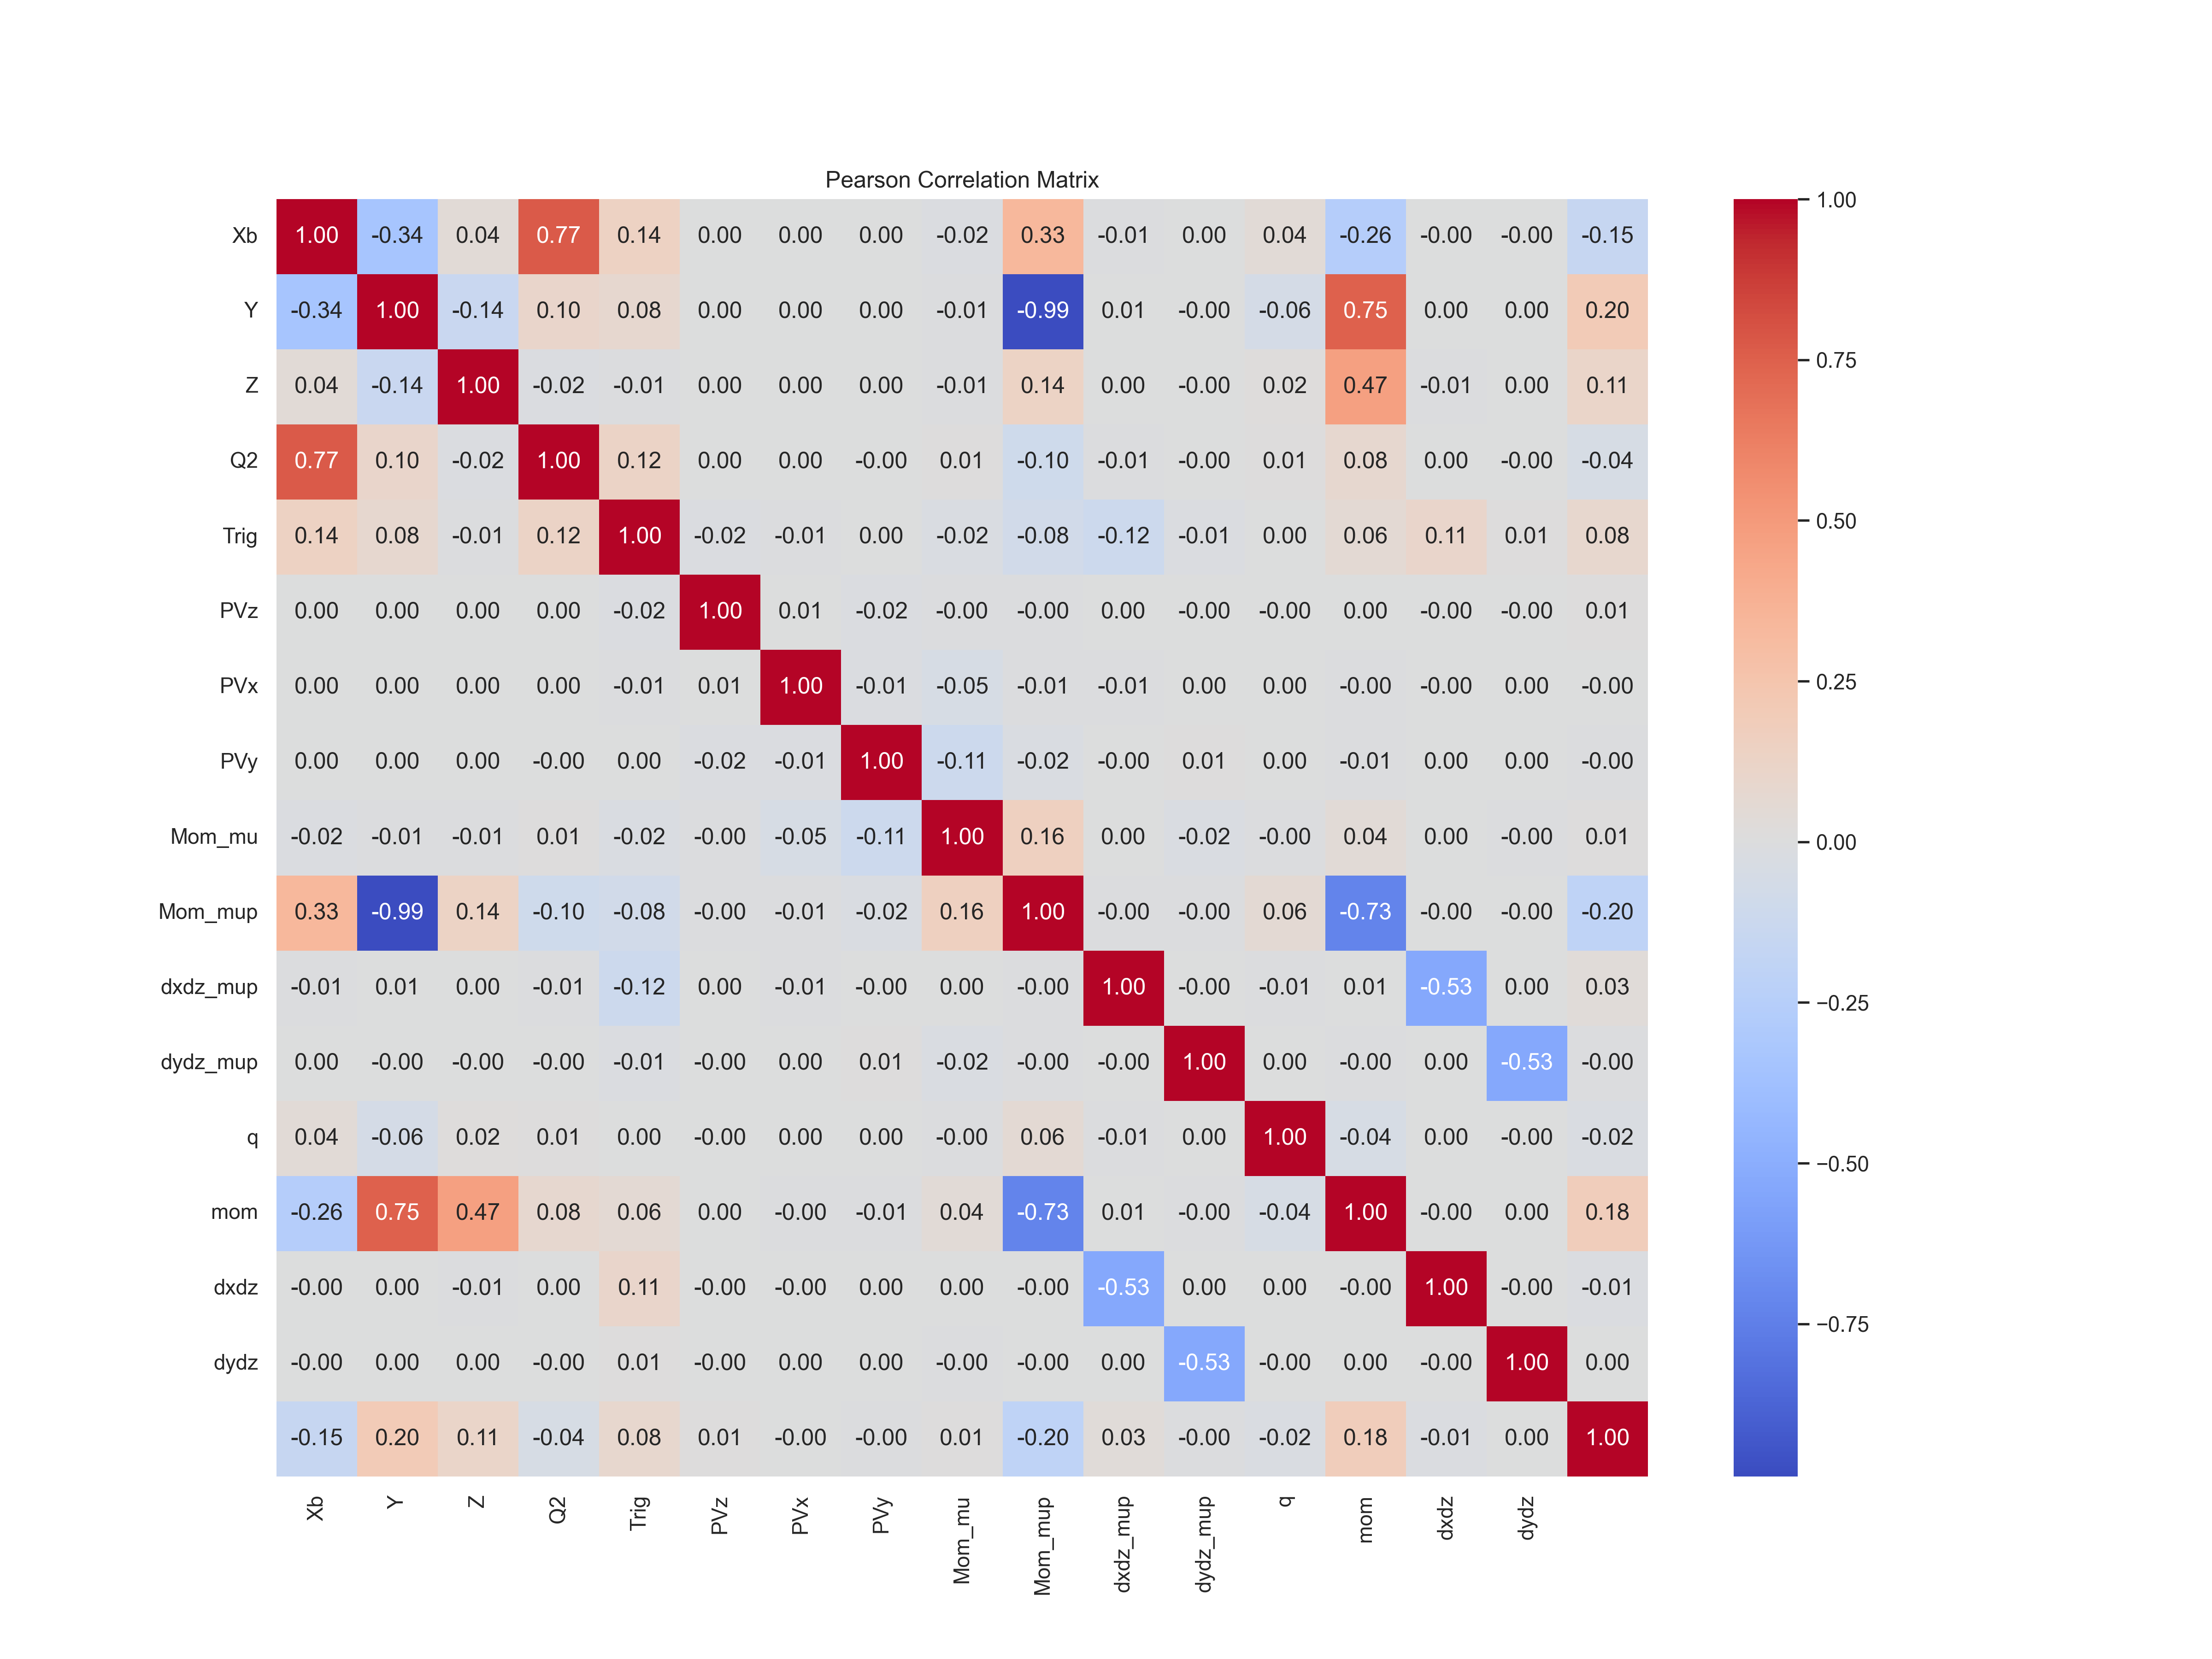
\includegraphics[width=0.9\textwidth]{graphs/hadron_correlation_matrix.png}
    \caption{Correlation Matrix for the Hadron Events}
    \label{fig:hadron_correlation_matrix}
\end{figure}


As seen in the figures above, there is a high correlation between $Y$ and $Mom_{mup}$, with
a pearson correlation coefficient of -0.99 for both types of events. Therefore, one of them can be removed from the training
of the Neural Network. Since $Mom_{mup}$ and $Y$ have the same correlation coefficient, we decided to remove $Mom_{mup}$ from the training of the Neural Network,
since from the physics point of view, $Y$ is more important than $Mom_{mup}$, since it is the variable that gives us the virtual photon energy fraction of the initial momentum. 

\subsubsection*{Weighting}
As mentioned before, the number of events for each of the files is different, since the Monte Carlo data has more events than the reconstructed data.
Hence, we had to balance the data for the training and testing of the Neural Network. This was done by weighting the events, so that the number of events
assigned to the training and testing set data as the same proportion of accepted and rejected events as the original data. Avoiding that when we split 
80\% of the data for training and 20\% for testing, we would have a different proportion of accepted and rejected events in the training and testing set data.
The weighting was done by calculating the ratio between the number of accepted and rejected events in the original data, and then multiplying the number of events.


\subsection*{Neural Network Models}

\subsubsection*{Models Architecture, Hyperparameters and Metrics}
For the Neural Networks models we used the PyTorch framework, which is an open source machine learning library based on the Torch library, used for applications such as computer vision and natural language processing.
For the models architecture, two different models were used, one with 3 hidden layers, two GELU activation functions and two dropout layers, and another with 6 hidden layers, 5 GELU activation functions and 3 dropout layers.
The choice of the number of hidden layers and the number of neurons in each layer was done by trial and error, and the same applies to the choice of the dropout rate. 
The GELU activation function was chosen because it is the one that gave the best results, and the same applies to the choice of the optimizer, which was the Adam optimizer.
These two models were chosen because they are the ones that gave the best results and also because there was the need to see the difference between a not so deep model and a deeper model.
The hyperparameters used for the training of the models were the following:
\begin{itemize}
    \item Learning Rate: 0.01
    \item Epochs: 10
    \item Batch Size: 1
\end{itemize}

For the loss function, we used the Binary Cross Entropy Loss, which is the most common loss function used for binary classification problems.
Despite the fact that this set of data might be familiar with a binary classification problem, since we are trying to predict if an event will be accepted or rejected,
we are not doing a binary classification problem, since we are not trying to classify the events, but rather predict the acceptance of the COMPASS/AMBER.
Therefore, there was no need to round the output of the Neural Network to 0 or 1, since the output of the Neural Network is a number between 0 and 1, which represents the probability of the event being accepted.
During the training of the models, we printed the accuracy and the loss as metrics to evaluate part of the performance of the models.
But since the accuracy and loss are not the best metrics to evaluate the performance of the models in this type of problems, the chi-squared test was used to evaluate the performance of the models.
The chi-squared test is a statistical hypothesis test that is used to evaluate how well a set of data fits a model. In this case, the model is the Neural Network, and the data is the data used for the training and testing of the Neural Network.
For this particular case, the chi-squared was applied to a 2D histogram, where the $x_axis$ is the $X$ variable and the $y_axis$ is the $Y$ variable.
The chi-squared used was defined as:

\begin{equation}
    \chi^2 = \sum_{i=1}^{N} \frac{(\frac{r}{g} - A_{nn})^2}{err}
\end{equation}
    
where $O_i$ is the observed value and $E_i$ is the expected value. The expected value is the value that the model predicts, and the observed value is the value that the data has.


\subsubsection*{Training, Testing and Results}

\section{Conclusion}



\end{document}